\documentclass[a4paper,10pt,twoside,openany]{book}

\usepackage[utf8]{inputenc}
\usepackage[T1]{fontenc}
\usepackage[english]{babel}
\usepackage[margin=22mm,inner=21mm,outer=19mm]{geometry}
\usepackage{microtype}
\usepackage{graphicx}
\usepackage{hyperref}

\newcommand{\mr}{\textsc{MR}}
\newcommand{\mrmac}{\textsc{MRMAC}}

\hypersetup{
  colorlinks=true,
  linkcolor=black,
  urlcolor=black,
  pdftitle={MR Technical Manual},
  pdfauthor={Dr. Michael 'iDoc' Raus}
}
\setlength{\emergencystretch}{4em}

\title{\mr{} Technical Manual\\\large A technical history of boundaries, speed, and extensibility}
\author{Dr.\ Michael 'iDoc' Raus}
\date{16 July 2026}

\begin{document}
\frontmatter
\begin{titlepage}
\begin{center}
\vspace*{\fill}
{\LARGE \mr{} Technical Manual\par}
\vspace{0.5\baselineskip}
{\large A technical history of boundaries, speed, and extensibility\par}
\vspace{3\baselineskip}
{\large Dr.\ Michael 'iDoc' Raus\par}
\vspace{2\baselineskip}
{\large 16 July 2026\par}
\end{center}
\vspace*{\fill}
\end{titlepage}

\chapter*{Preface}
\addcontentsline{toc}{chapter}{Preface}

This is neither a class catalogue nor retrospective self-congratulation. It
explains why \mr{} is built differently from a conventional terminal editor in
several important respects, which experiments were abandoned, and which limits
remain despite the successes. Its sources are the repository, architecture
contracts, planning documents, Kanban entries, and version history. Where
those sources do not support a claim, this manual does not make it.

The MRMAC Reference Manual documents the language and its primitives. This
book tells a different story: how document handling, runtime, UI, and user
customisation became one system whose parts do not quietly take ownership of
one another.

\tableofcontents

\mainmatter
\part{Why \mr{} exists}

\chapter{Not another editor}

\mr{} began with the intention of carrying the character of Multi-Edit
forward, not as a nostalgic surface but as a way of working. An editor should
be immediate, keyboard-capable, and at home in a terminal. At the same time,
it should not treat large files, many windows, build output, and automation as
foreign bodies.

This heritage produced several non-negotiable goals: speed, a practically
unbounded workspace, reliable editing operations, extensibility and
customisation by the user, and responsiveness under load. The close
relationship between \mrmac{} and the compiled application is therefore not
an item at the end of a plugin list. It is part of the product's definition.
Decoupling matters just as much: a document may be edited while derived work
is being produced, but a background result must not write itself into a screen
that has moved on in the meantime.

The guiding principle is consequently not \emph{as many features as possible},
but \emph{as much productive power as possible without sacrificing control}.
Each chapter asks a concrete question: which technical problem threatened that
goal, what idea shaped the solution, and where did \mr{} deliberately reject a
seemingly convenient alternative?

\chapter{Standing on the shoulders of others}

\mr{} does not attempt to carve every wheel from scratch. Its distinctive
character comes precisely from the boundary between inherited foundations and
its own semantics.

The working model comes from Multi-Edit and the MEMAC tradition: windows,
blocks, macros, and personal interaction should be ordinary parts of editing
rather than exceptional add-ons. \mrmac{} preserves that lineage, while being
its own compiled, in-memory runtime.

Magiblot's TVision provides the terminal-native object world. TVision owns
focus, Z order, event routing, view lifetime, dialogs, and drawing dispatch.
\mr{} extends that world through its intended mechanisms instead of placing a
second screen model or event loop beside it. The dependency is maintained as
an upstream subtree with a small patch queue. This is a deliberate
relationship: upstream remains identifiable and local changes remain
reviewable.

The frequently proposed alternative is not really TVision \emph{or}
\texttt{ncursesw}. \mr{} links against \texttt{ncursesw}; it is part of the
terminal platform beneath TVision. The actual choice was TVision rather than
building a window, focus, dialog, and drawing system directly on bare curses.
For an editor with virtual desktops and a long Multi-Edit UI tradition, that
was a useful trade: less invented infrastructure, more energy for documents
and runtime behaviour.

PCRE2 supplies Perl-compatible regular-expression semantics for search and
multi-file work. POSIX supplies, among other things, \texttt{mmap}, processes,
and pipes. Pango and Cairo support PDF export. These components are not hidden
MR subsystems. Each solves a clearly bounded problem; responsibility for
placing its results in the editor model remains with \mr{}.

\part{The document as workspace}

\chapter{A gigabyte file in five milliseconds}
\label{ch:large-files}

The striking number needs to be told accurately. The \texttt{enwik9} file
used in the repository contains exactly 1,000,000,000 bytes and 13,147,025
lines. On the measured development machine, \mr{} makes this document
available as an editable document in about five milliseconds.

That does not mean that a gigabyte is copied from storage and fully analysed
in five milliseconds. The number is the measured \emph{mapped load} time.
\mr{} opens a regular file as a private, read-only memory mapping and builds
its logical document state on top of that mapping. The operating system brings
pages in on demand; the editor does not first copy the original into a mutable
string.

A Piece Table sits above the mapping. The original remains the source of
pieces, new input goes into the add buffer, and the logical order is expressed
as references to those sources. An edit therefore does not move a gigabyte of
text. It changes piece boundaries and adds new data to the add buffer. This
model serves more than load time: it makes editing, snapshots, undo boundaries,
and later derived work variations of the same data economy.

Figure~\ref{fig:piece-table-snapshot-boundary} makes the ownership boundary
explicit. A background task receives a versioned read snapshot, never the
mutable live object. It may return a derived result or a staged edit, but it
cannot adopt that work itself.

\begin{figure}[htbp]
  \centering
  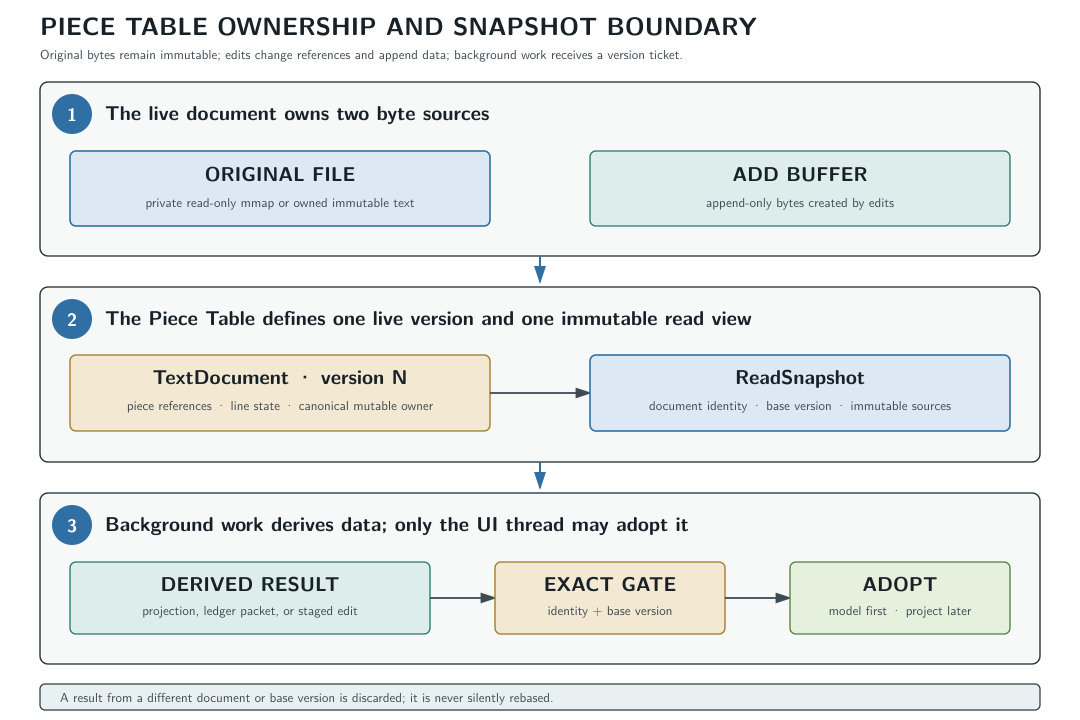
\includegraphics[width=\textwidth]{assets/mr-piece-table-snapshots.pdf}
  \caption{Piece Table ownership and the snapshot boundary. The mapped or
  owned original and append-only buffer are the sources of the live document.
  Background work receives a versioned \texttt{ReadSnapshot}; only the UI may
  adopt a result whose document identity and base version still match.}
  \label{fig:piece-table-snapshot-boundary}
\end{figure}

The line index may then warm up in a controlled manner. Until an exact total is
available, the editor uses a justified estimate; navigation and the visible
area remain usable. The enwik9 milestone was therefore not satisfied by a fast
``opened'' message. It required responsive loading, scrolling, jumping,
editing, and discarding. Only that sequence demonstrates that the fast start
is not a demonstration effect.

\section{Non-blocking deferred scans}

Deferred scanning is not one pass over the document. The editor runs separate
line-index, syntax, fold, and minimap pipelines. Each pipeline captures a
versioned \texttt{ReadSnapshot}, defines a half-open line interval
\([top,bottom)\), and submits work to the appropriate coprocessor lane. The UI
thread does not wait for that work. It continues to draw from the currently
valid projection while the worker produces a typed result.

The line-index pipeline is the global forward scan. A worker invocation calls
\texttt{warmLineIndexChunk} with a budget of two index strides. The returned
\texttt{LineIndexWarmupData} contains the accumulated
\texttt{LineIndexCheckpoint} entries, \texttt{lazyIndexedOffset},
\texttt{lazyIndexedLine}, the completion flag, and the total line count when
known. An accepted result schedules the next bounded invocation until the
indexed boundary reaches EOF. BOF is already the fixed index origin; this
pipeline does not perform a second backward warm-up. Backward navigation uses
the available checkpoints and the reverse line-break primitive.

Viewport-derived pipelines use a different topology. Their scan interval is a
bounded window around the active viewport, not necessarily the complete
document. The viewport is the focus interval, the lower scan bound points
towards BOF, and the upper bound points towards EOF. Moving the viewport may
therefore replace a pending request with a new window. A request already
covering the required interval is reused.

Fold acquisition divides the requested interval into chunks of 256 lines. It
constructs the focus chunk and the adjacent chunks above and below it, bounded
by \texttt{scanTopLine} and \texttt{scanBottomLine}. Before structural
evaluation, the chunks are ordered by their document position and concatenated.
This ordering is mandatory: nesting, closing markers, sibling continuations,
and branch levels depend on the state produced by preceding lines. The fold
result retains the actual scan bounds, the source line texts, fold spans,
gutter branches, and the maximum visible nesting width. A complete outline is
available only when the retained fold interval covers BOF through EOF; a
viewport-local result is explicitly a partial outline source.

Minimap acquisition starts at the viewport anchor inside its sampling window.
It obtains line texts first from the anchor towards the window's EOF-side end
with \texttt{nextLine}, then from the anchor towards the BOF-side start with
\texttt{prevLine}. It does not retain those texts as a second document model.
The worker reduces them to Braille cell patterns and records, for every minimap
row, the corresponding document-line start and end. The fixed sampling window
therefore supplies both pixels and the inverse mapping required for viewport
and overlay placement.

Syntax warm-up is forward because lexical state flows from an earlier line to
a later line. For a stateful language, a request above the viewport locates the
nearest valid syntax checkpoint or a bounded prelude towards BOF. Analysis then
runs forward through the visible range and continues in bounded prefetch bursts
towards EOF. Every cached line retains its input state, token runs, and output
state. A cached prefix is reusable only while the state chain remains equal;
the first mismatch terminates that reusable prefix.

Figure~\ref{fig:coprocessor-warming-projections} shows the four derived
projections at one viewport position together with their task telemetry. The
numbered callouts identify rendered consumers and instrumentation, not
additional scan stages.

\begin{figure}[htbp]
  \centering
  \begingroup
  \setlength{\unitlength}{0.00098\textwidth}
  \begin{picture}(1000,540)
    \put(0,0){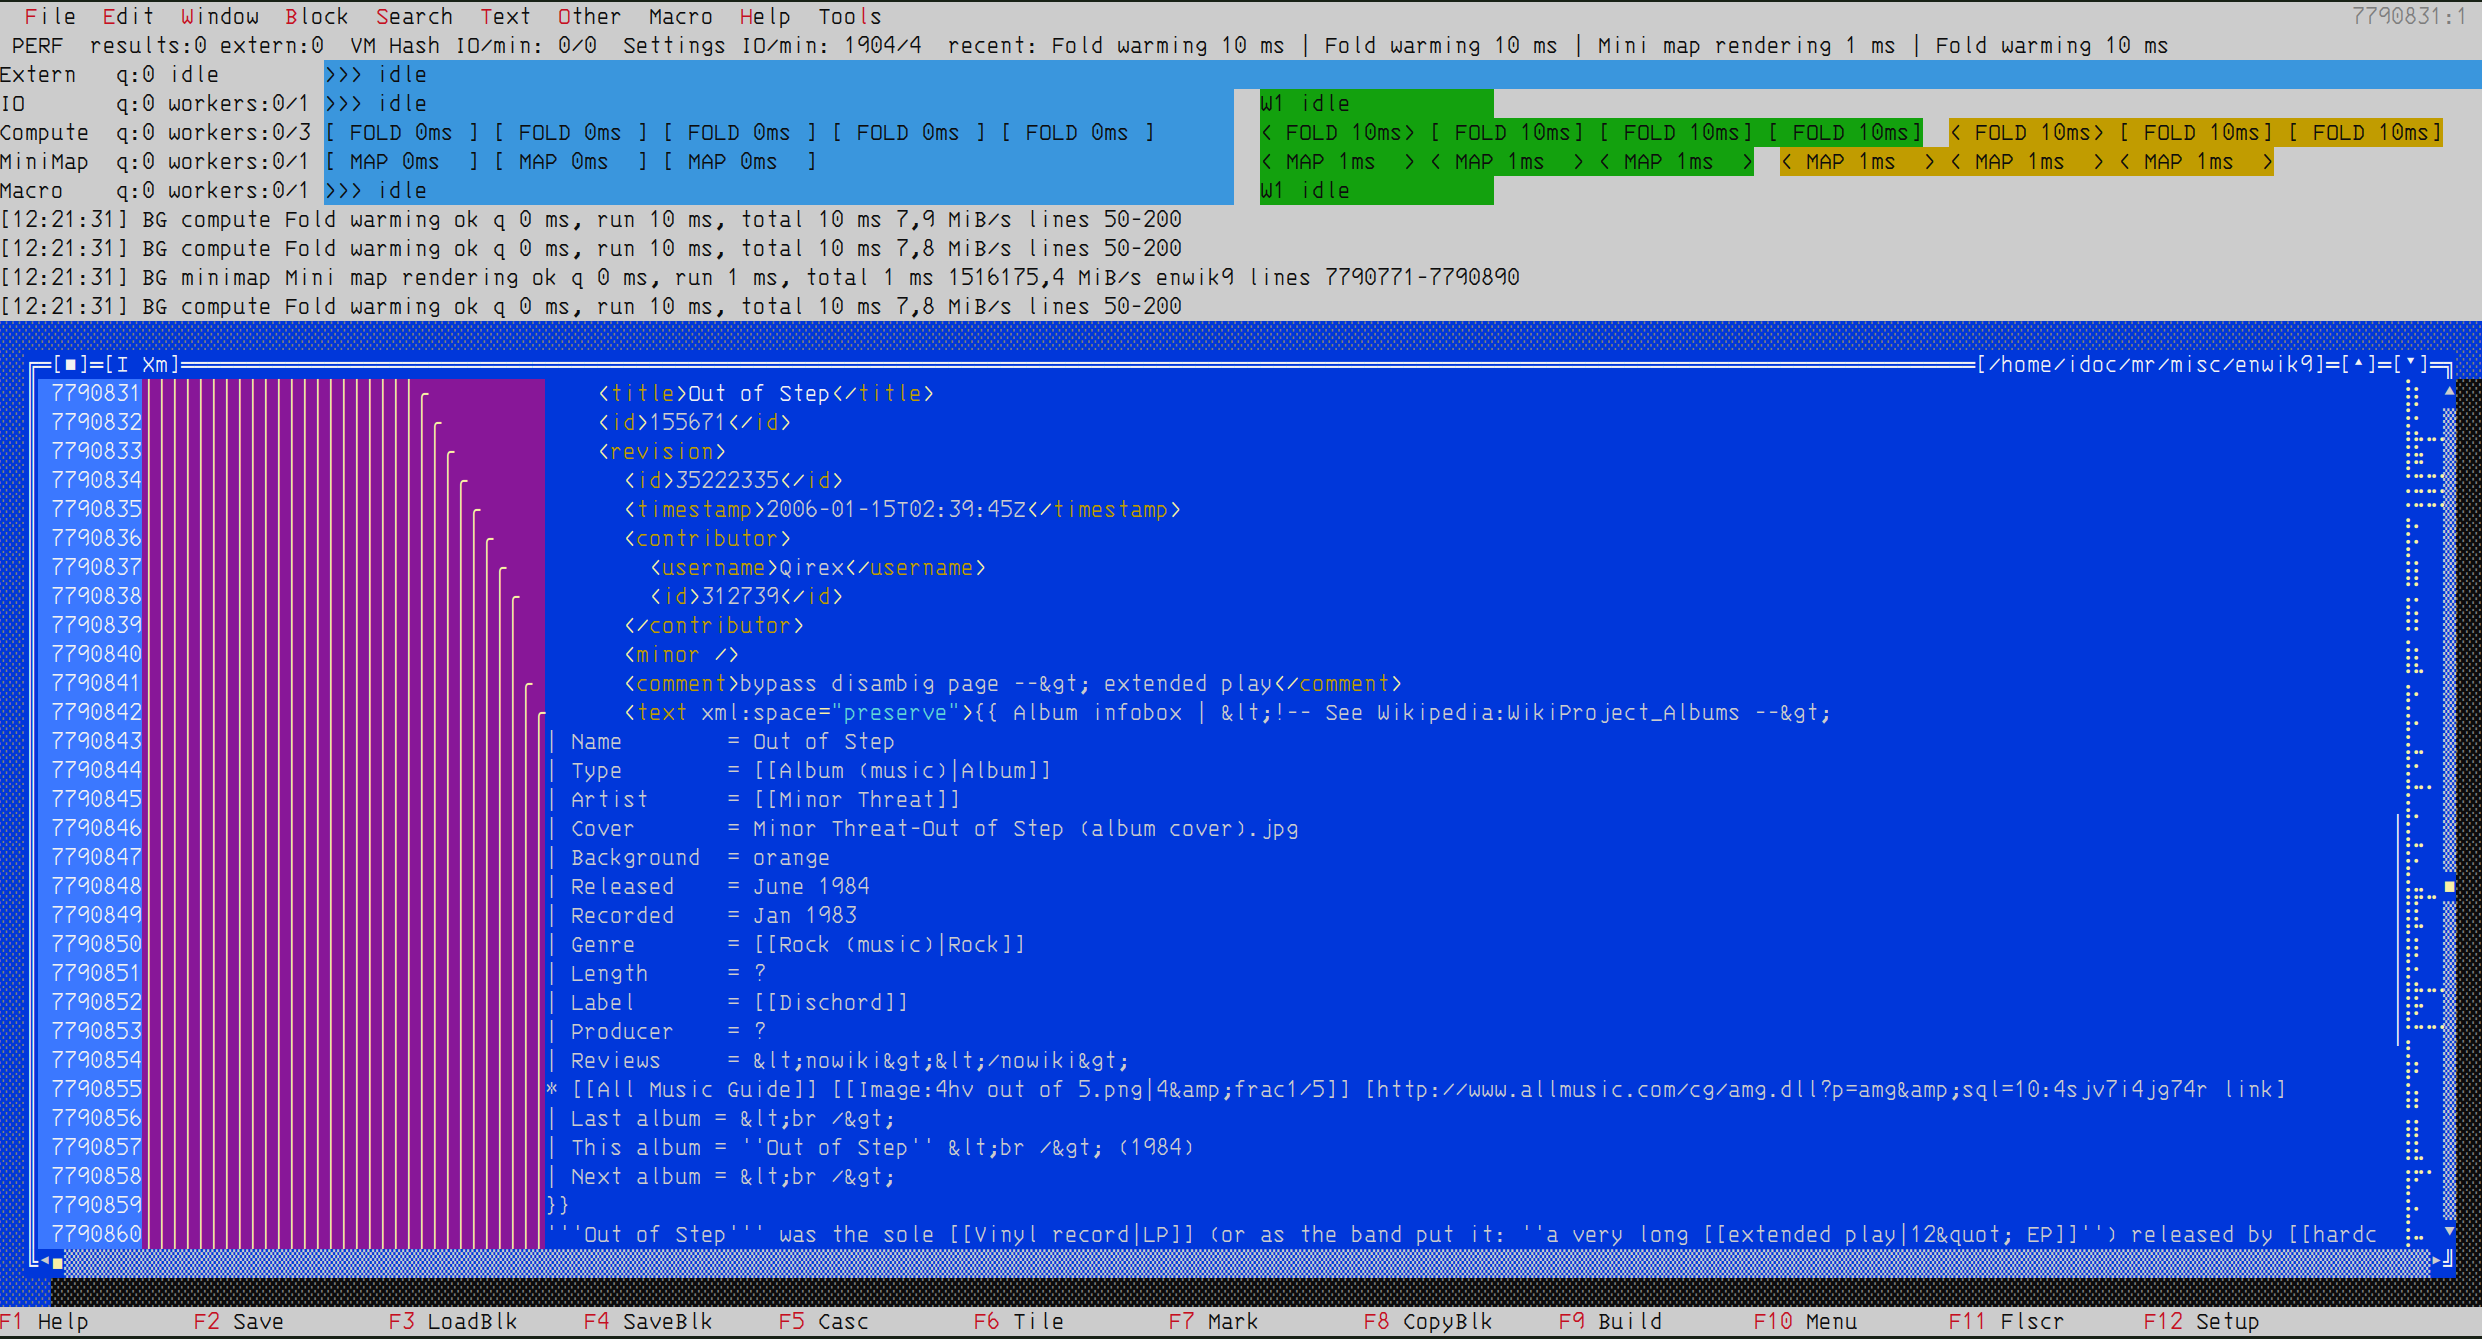
\includegraphics[width=0.98\textwidth]{../pngsjpegs/COPRO_warming.png}}
    \put(790,500){\makebox(0,0){\Large\textcircled{\normalsize\textbf{1}}}}
    \put(45,360){\makebox(0,0){\Large\textcircled{\normalsize\textbf{2}}}}
    \put(190,330){\makebox(0,0){\Large\textcircled{\normalsize\textbf{3}}}}
    \put(520,360){\makebox(0,0){\Large\textcircled{\normalsize\textbf{4}}}}
    \put(960,300){\makebox(0,0){\Large\textcircled{\normalsize\textbf{5}}}}
  \end{picture}
  \endgroup
  \caption{Deferred projections while viewing enwik9 near line 7,790,831:
  (1) coprocessor task and timing telemetry, (2) line-number projection,
  (3) fold spans and branch continuations in the gutter, (4) syntax token
  projection in the editor body, and (5) the viewport-anchored Braille
  minimap.}
  \label{fig:coprocessor-warming-projections}
\end{figure}

\section{Retained information and render consumers}

The payloads and caches preserve only the information required by their
consumers:

\begin{center}
\small
\setlength{\tabcolsep}{3pt}
\begin{tabular}{|p{0.18\textwidth}|p{0.42\textwidth}|p{0.30\textwidth}|}
  \hline
  \textbf{Projection} & \textbf{Retained information} & \textbf{Direct consumer} \\
  \hline
  Line index & byte/line checkpoints, indexed byte and line frontier,
  completion state, exact total when complete & line numbers, byte-to-line and
  line-to-byte navigation, scrollbar and document metrics \\
  \hline
  Syntax & line start, \texttt{stateIn}, token runs with column, length and
  token class, and \texttt{stateOut} & coloured editor text and the state
  checkpoint chain for subsequent lines \\
  \hline
  Folding and outline & scan bounds, line texts, fold start/end, nesting
  level, source kind, open state, sibling continuation, gutter branches and
  visible gutter width & fold gutter, closed-line projection and partial or
  complete outline generation \\
  \hline
  Minimap & total line count, sampling-window bounds, viewport width, Braille
  row patterns and document-line interval per row & minimap cells, viewport
  marker and line-based overlays \\
  \hline
  Performance view & task kind, lane, queue/run/total duration, throughput and
  processed line range & observability only; never a semantic input to an
  editor projection \\
  \hline
\end{tabular}
\end{center}

Every result remains provisional until dispatch. Adoption requires the pending
task identifier, document identity, base version, and---where applicable---the
language and render geometry to match the current editor state. A mismatch
discards the result. The UI thread is the only point at which a valid result is
installed into a derived-state cache and made visible.

\section{Moving windows and the warmed-range ledger}
\label{sec:warmed-range-ledger}

Large-file syntax warm-up maintains one active request window and a separate
record of all accepted warm intervals. \texttt{WarmupState} identifies the
currently submitted \([topLine,bottomLine)\) task.
\texttt{PrefetchState} records the EOF-side target and the line reached for the
current viewport. A large cursor jump recomputes both bounds from the new
viewport; it does not translate the old window through the document.

Only one viewport-local syntax task for the same document, version, and
language may be pending. If the cursor moves while that task is running,
\texttt{scheduleSyntaxWarmupIfNeeded} defers the new submission. Dispatch first
applies or rejects the pending result and clears its task identifier; the
subsequent continuation evaluates the then-current viewport and submits its
window. An identical recently completed request is additionally suppressed by
the 180 millisecond large-file burst debounce.

Accepted line results are stored in the token cache and their produced line
interval is passed to \texttt{rememberWarmedLineRange}. The valid-range ledger
is owned by document identity and syntax language. Cursor movement does not
clear it, so a large jump can leave multiple disjoint intervals. Each insertion
is sorted and normalized: overlapping or touching intervals are merged, while
gaps remain explicit.

A ledger hit is necessary but not sufficient for reuse. The requested interval
must be covered without a gap, and \texttt{syntaxCachedCoveragePrefix} must
also reproduce the cached \texttt{stateIn}/\texttt{stateOut} chain from the
required initial state. Full coverage suppresses the worker request. Partial
coverage removes the verified prefix and submits only the missing tail; the
accepted tail is then merged into the ledger. An edit truncates valid ranges,
token entries, and checkpoints from the first affected line. A document or
language change clears the ledger. Worker adoption still performs the
independent task, document, version, and language checks.

Figure~\ref{fig:deferred-scan-windows} shows the window movement and range
normalization for an initial viewport, a large cursor jump, and an overlapping
return request.

\clearpage
\begin{figure}[htbp]
  \centering
  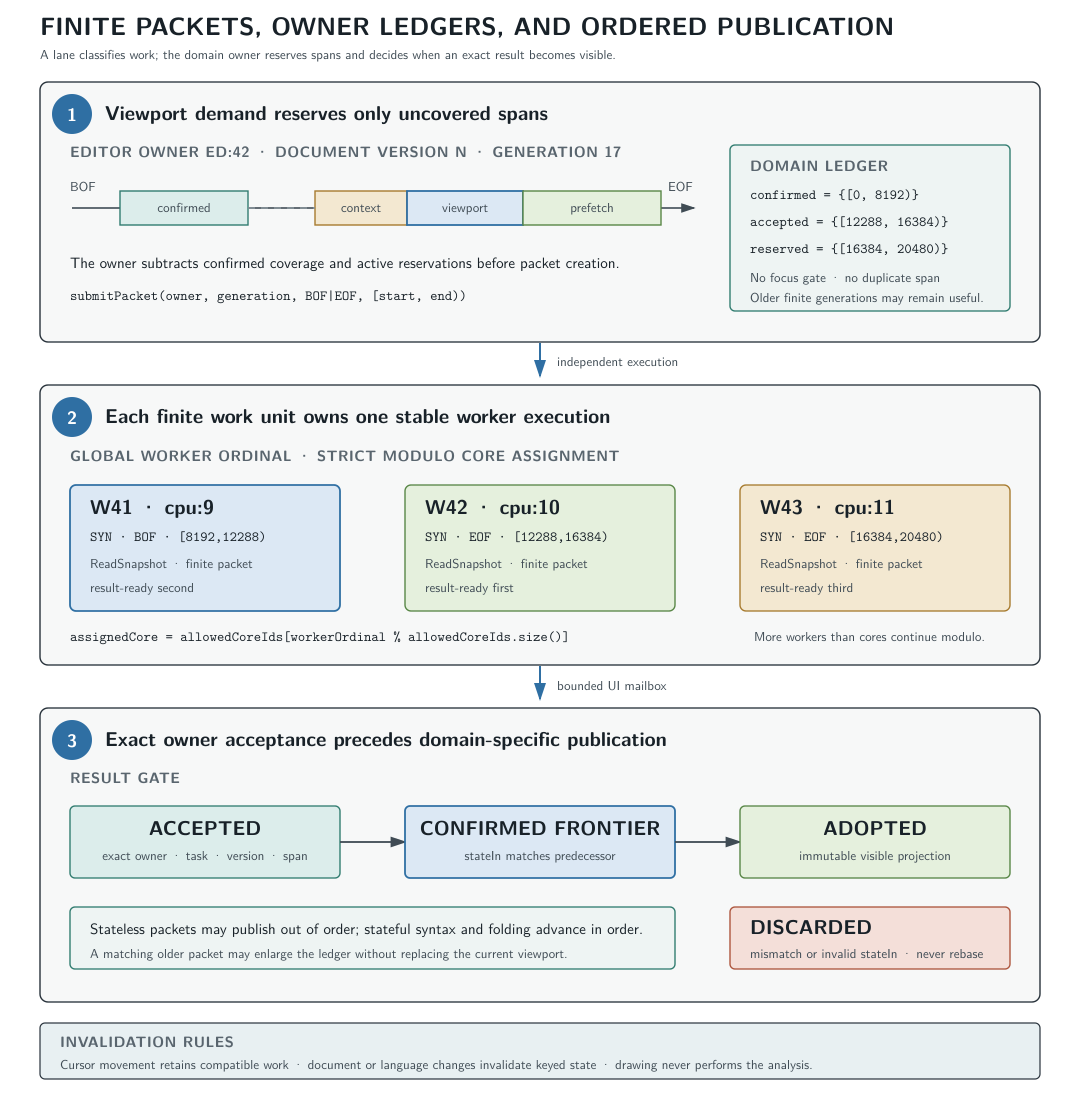
\includegraphics[width=0.92\textwidth]{assets/mr-deferred-scan-windows.pdf}
  \caption{Viewport-local syntax warm-up and its persistent range ledger.
  Step 1 records the first produced interval. Step 2 relocates the active scan
  window after a cursor jump while retaining the disjoint earlier interval.
  Step 3 verifies a cached prefix, scans only the missing tail, and merges the
  accepted result with the touching interval.}
  \label{fig:deferred-scan-windows}
\end{figure}

\section{Line-break scan primitives}

Line navigation, line numbering, index warm-up, and Piece Table scans require
the same three operations: locate the next line break, locate the previous line
break, and count line breaks in a byte range. These operations are implemented
in the line-index core. On x86 builds with SSE2, the core loads sixteen bytes at
a time, compares them with carriage return and line feed, and converts the
resulting bit masks into positions and counts. A scalar implementation is the
fallback for platforms without the vector path.

The scanner carries CRLF state across vector blocks and handles the scalar
tail, preserving the same line model at vector and chunk boundaries. The
counting primitive operates on direct mapped text and on individual Piece Table
chunks; the direct path also uses vector search in both directions. A large
direct document may be divided into line-aligned warm-up chunks, while SIMD
performs the inner scan of each chunk. All derived pipelines therefore consume
one line model rather than maintaining feature-specific text indexes.

\chapter{Derived work must not stop the editor}
\label{ch:coprocessor-derived-work}

The coprocessor is a lane scheduler with one result boundary, not a general
executor from which a worker may call back into the application. It separates
derived CPU work, minimap projection, macro execution, ordered command I/O,
and independent live sources because these workloads have different ordering
and starvation requirements. Figure~\ref{fig:coprocessor-lanes} shows the
complete path from submission to an accepted derived state. Markers 1--5 in
the figure identify the concrete lanes described below.

\clearpage
\begin{figure}[p]
  \centering
  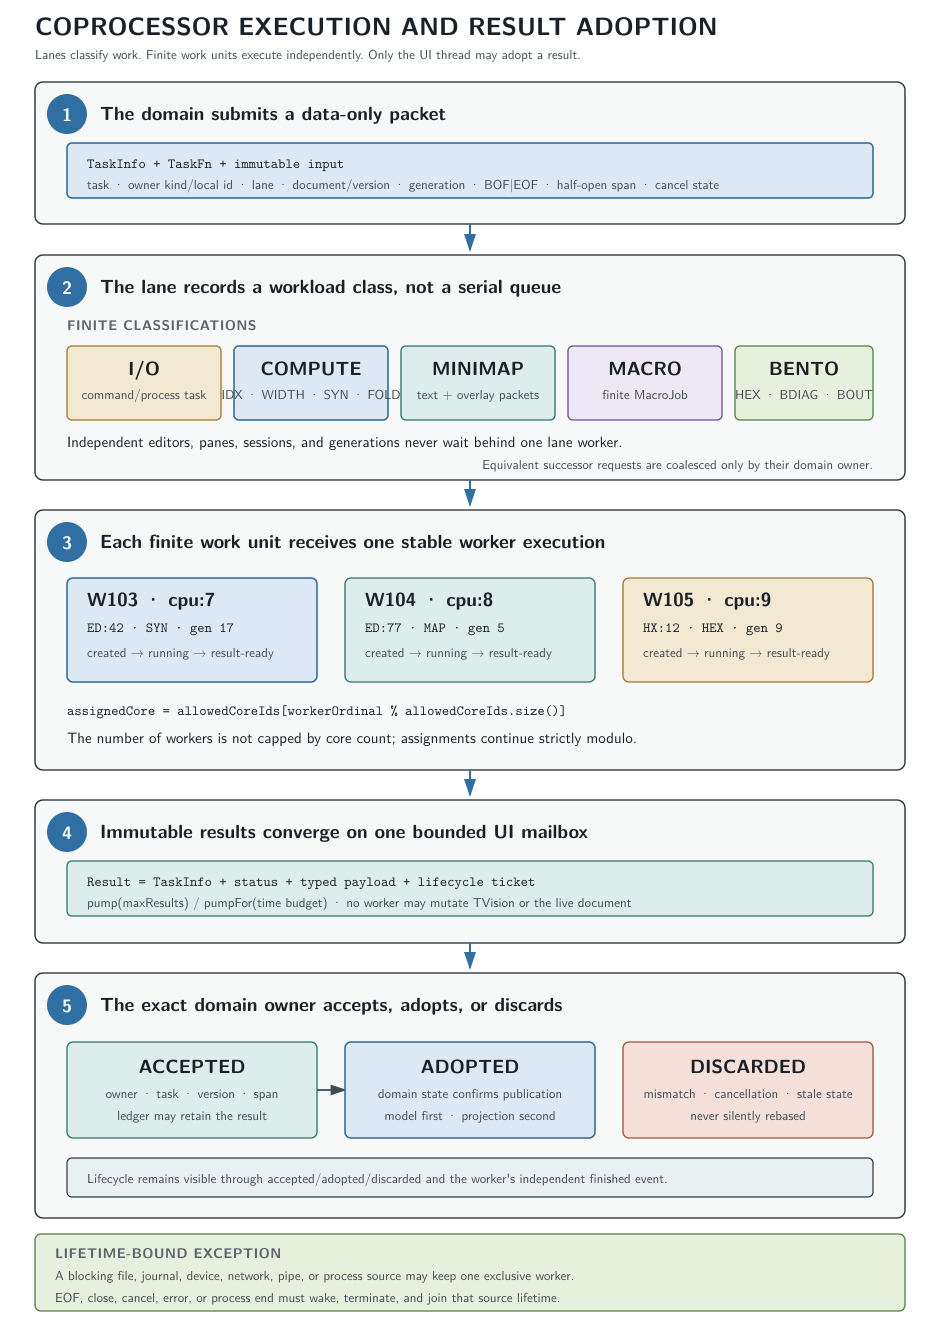
\includegraphics[width=0.94\textwidth]{assets/mr-coprocessor-lanes.pdf}
  \caption{Coprocessor execution and result adoption. A submission carries a
  data-only task envelope into one lane. Workers produce typed results but do
  not mutate TVision state. All lanes converge on one result mailbox; the UI
  thread drains it within a count or time budget and delegates the final
  acceptance decision to the owning domain.}
  \label{fig:coprocessor-lanes}
\end{figure}
\clearpage

\section{Task envelope and scheduling boundary}

\texttt{submit} and \texttt{submitCoalesced} construct a \texttt{TaskInfo}
with a unique task identifier, lane, task kind, document identity, base
version, diagnostic label, and shared cancellation flag. The request also
contains the task function, its submission timestamp, and---for compute
work---its priority. Document-derived submitters capture the coherent read
snapshot or copied input on which the task operates; \texttt{documentId} and
\texttt{baseVersion} are the ticket by which the eventual result is compared
with live state, not permission for the worker to read the view.

If a non-empty coalescing key is supplied, a newer request removes queued,
not-yet-running requests with the same task kind and key from that lane. An
active request is not pre-empted by coalescing. \texttt{MacroJob} is explicitly
excluded because two macro executions are distinct events even when their
labels or inputs resemble one another. Current editor warm-up producers also
keep their own pending-task discipline, as described by the moving-window
mechanics in Chapter~\ref{ch:large-files}.

Worker cardinality belongs to a lane, not to the coprocessor as a whole. The
four static lanes provide four through six workers in total: one each for
\texttt{Io}, \texttt{MiniMap}, and \texttt{Macro}, plus one through three for
\texttt{Compute}. Every registered external source can add its own worker.

Before executing a task function, every worker activation binds the current
worker thread round-robin to one CPU from the process affinity mask. One task
therefore executes on one eligible CPU at a time, but neither the lane nor the
worker owns that CPU exclusively or permanently. The next activation advances
the shared affinity slot and may place the same worker on another CPU. The task
function receives both the shared task cancellation state and a
\texttt{stop\_token}; cancellation remains cooperative.

\section{Lane responsibilities and use cases}

\subsection{1 --- I/O lane}

The static \texttt{Io} lane is one FIFO with one worker. Its current application
use is ordered external-command and build-process execution initiated by the
command router. A task may post \texttt{ExternalIoChunkPayload} results while
the process is running and finally return an
\texttt{ExternalIoFinishedPayload} containing exit, signal, build-context, and
post-build information. Serial execution is intentional here: conventional
command I/O has one application-level ordering point. Independent permanent or
streaming sources use lane 5 instead.

\subsection{2 --- Compute lane}

The \texttt{Compute} lane owns three FIFO priority queues. Line-index warm-up
and indicator timing are high priority. Syntax, folding and outline acquisition,
save-normalisation warm-up, and file comparison are normal priority. Custom
work, currently including the macro-delay helper, is low priority. Within one
priority the queue order remains FIFO.

Worker count follows the reported hardware concurrency: one worker below four
hardware threads, two from four through seven, and three from eight upwards.
On a multi-worker lane, if high-priority work is already active while normal
work is waiting, the next selection admits normal work instead of allowing
high-priority tasks to occupy every available worker. High work retains the
first preference; normal derived work retains forward progress.

The resulting payloads are domain-specific: line checkpoints, syntax runs and
state, fold structure, normalisation metadata, diff hunks, or an indicator
generation. The deferred scan windows and their retained information are the
principal editor use case detailed in Chapter~\ref{ch:large-files}.

\subsection{3 --- MiniMap lane}

The \texttt{MiniMap} lane is a dedicated FIFO with one worker and accepts
\texttt{MiniMapWarmup}. It prevents repeated minimap sampling from competing
with line-index and syntax work in the compute queues. Its payload contains the
sampling geometry, total and sampled line ranges, Braille row patterns, and
the document-line start and end represented by each minimap row. Chapter~\ref{ch:minimap}
describes how this derived projection is rendered and overlaid.

\subsection{4 --- Macro lane}

The \texttt{Macro} lane is a dedicated FIFO with one worker. Background and
staged-background Execution Sessions submit \texttt{MacroJob}; jobs are not
coalesced, and the single worker preserves their lane order. An ordinary
background result returns logs and UI-command requests as data. A staged result
additionally carries the edit transaction, runtime values, cursor and selection
state, a conflict snapshot, and deferred UI commands. None of those objects is
installed by the worker. Chapters~\ref{ch:execution-sessions}
and~\ref{ch:macro-staging} describe session routing and staged commit.

\subsection{5 --- Dynamic external-source lanes}

\texttt{Extern} does not denote one global fifth queue. Registering a file,
journal, device, network, or pipe source creates an external-source state with
its own \texttt{LaneState}; the single worker for that source is started lazily
on its first \texttt{submitExternal}. Consequently, a blocked device or quiet
file cannot serialize unrelated live sources behind itself.

An external task uses \texttt{ExternalIo}, with the source identifier carried
in the task's document-identity field and base version zero. Chunk results feed
the target live-log or communication buffer on the UI thread. The source state
also records received bytes, activity sequence, and a bounded stream sample for
the performance projection. Completion or failure releases and unregisters the
dynamic lane.

\section{Worker completion and the result mailbox}

The worker loop removes one request under the lane lock, records it as active,
performs the affinity placement, and invokes the task outside the lock.
Exceptions are converted into a failed \texttt{Result}; a cancellation observed
before execution produces a cancelled result. Completion records queue, run,
and total duration in microseconds. The active entry is then removed and the
result appended to the mutex-protected central FIFO. No lane has a private path
to the screen.

\texttt{pump(maxResults)} drains at most the requested count---eight by
default---whereas \texttt{pumpFor} stops after the supplied time budget once a
result has been handled. Both invoke the installed result handler on the UI
thread. The central \texttt{handleCoprocessorResult} performs payload dispatch;
it does not replace the owning domain's validation.

For line index, syntax, fold, minimap, and save-normalisation results, dispatch
locates matching editors and admits completed data only against the current
document and base version. The editor then applies its remaining task-ID,
language, geometry, or options checks. File Compare validates both document
versions through its Bento owner. A staged macro compares its captured conflict
state before committing. External chunks and indicator generations likewise
become visible only through their UI-thread owners. A mismatch clears the
pending task state and discards the payload; it is never rebased implicitly.

\section{Cancellation and observability}

\texttt{cancelTask} sets the shared flag and wakes all lane condition variables;
it cannot forcibly interrupt an arbitrary task function. Long-running task
functions must therefore inspect the cancellation flag or stop token at safe
points. Shutdown additionally requests worker stop and clears pending queues.

\texttt{snapshot} exposes the pending-result count and, for each static lane,
its worker count, active tasks with current queue/run times, and queued tasks.
External-source snapshots add kind, tag, running state, received bytes,
activity sequence, and stream sample. Completed results provide the measured
queue, run, and total times recorded by the performance view. These measurements
are observability outputs only; they never become semantic inputs to an editor
projection.

\chapter{A minimap with eight dots per character}
\label{ch:minimap}

The minimap is a viewport-anchored derived projection in an editor gutter. It
has two data paths. The coprocessor produces compact text-density patterns for
a bounded line window; the UI thread produces current overlay masks from
selection, search, edit, diagnostic, and File Compare state. The paths meet
only in \texttt{drawGutter}. Figure~\ref{fig:minimap-ui} identifies the three
visible components, and Figure~\ref{fig:minimap-function-flow} follows the
complete data path.

\begin{figure}[htbp]
  \centering
  \begingroup
  \setlength{\unitlength}{0.00098\textwidth}
  \begin{picture}(1000,543)
    \put(0,0){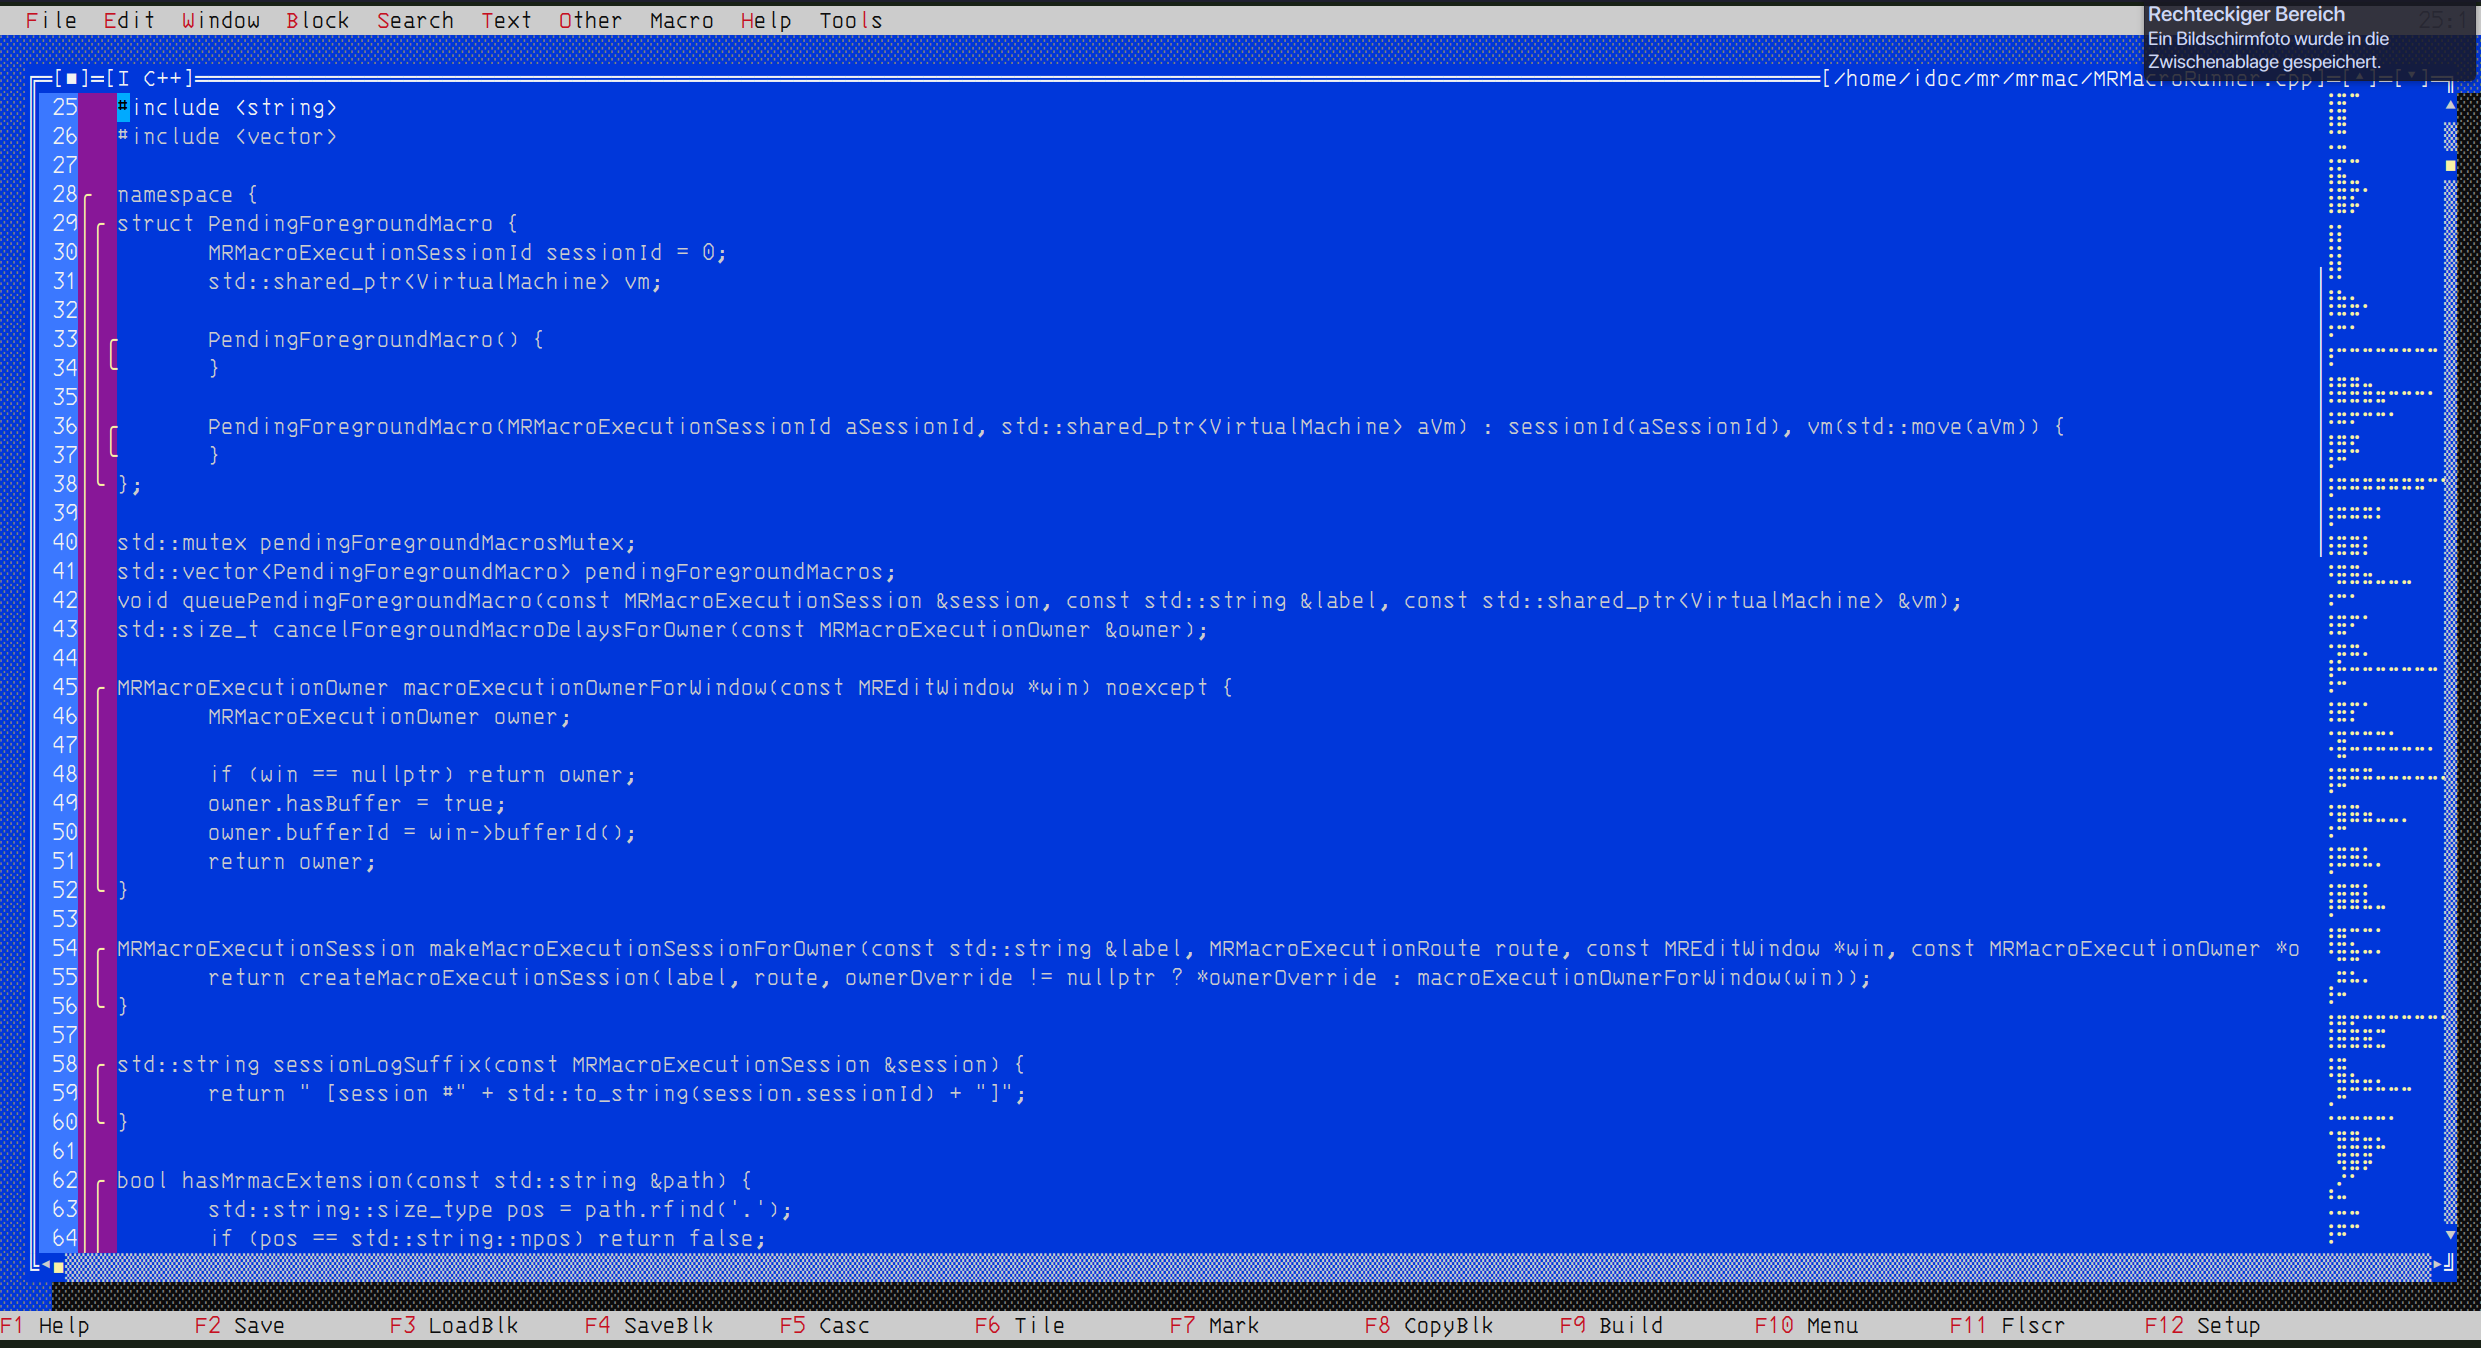
\includegraphics[width=0.98\textwidth]{../pngsjpegs/UI_minimap.png}}
    \put(946,365){\makebox(0,0){\Large\textcircled{\normalsize\textbf{1}}}}
    \put(925,315){\makebox(0,0){\Large\textcircled{\normalsize\textbf{2}}}}
    \put(982,260){\makebox(0,0){\Large\textcircled{\normalsize\textbf{3}}}}
  \end{picture}
  \endgroup
  \caption{Trailing minimap in the editor: (1) the Braille pattern body,
  (2) the separate viewport-marker column, and (3) the native TVision
  scrollbar. The minimap is a projection gutter, not a replacement input
  mechanism for the scrollbar.}
  \label{fig:minimap-ui}
\end{figure}

\clearpage
\begin{figure}[p]
  \centering
  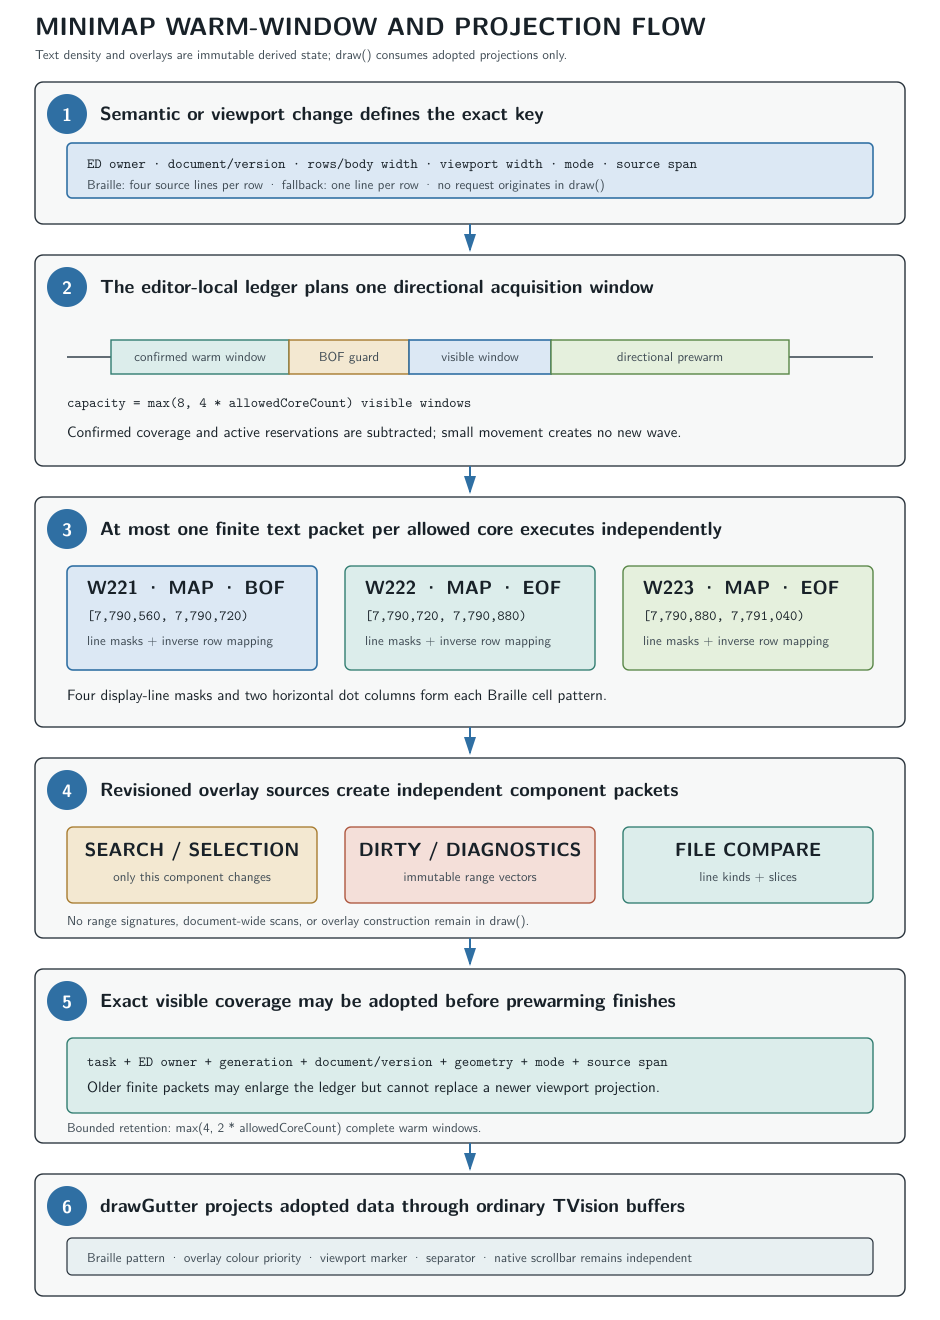
\includegraphics[width=0.94\textwidth]{assets/mr-minimap-function-flow.pdf}
  \caption{Minimap function flow. Geometry and a document/version ticket define
  the sampling request. The single-worker minimap lane reduces copied line
  text to Braille patterns. After UI-thread adoption, cached patterns and
  current overlay masks are combined into an ordinary TVision
  \texttt{TDrawBuffer}.}
  \label{fig:minimap-function-flow}
\end{figure}
\clearpage

\section{Geometry and the sampling window}

The effective edit settings select \texttt{OFF}, \texttt{LEADING}, or
\texttt{TRAILING}, a total minimap width from 2 through 20 cells, and a
single-cell viewport-marker glyph. \texttt{TextViewportGeometry} reserves the
body, marker, and optional separator columns. The body receives all but one
cell of the configured width; the marker occupies the independent
\texttt{infoX} column. The normal and File Compare palettes provide separate
colours without changing the generated patterns.

At the start of an editor draw, the renderer receives the body geometry,
visible text-row count, viewport width, top line, exact or estimated total line
count, document identity and version, and a read snapshot. Braille mode is used
only when TVision reports the full Braille glyph as one terminal cell. Otherwise
the renderer falls back to one block cell per sample.

\texttt{samplingWindowFor} assigns four source-line samples to every minimap
row in Braille mode and one in fallback mode. For $R$ minimap rows, its capacity
is therefore $4R$ or $R$ lines. A document no larger than that capacity uses
the interval $[0,totalLines)$. A larger document uses a capacity-sized window
centred on \texttt{topLine}, clamped first at BOF and then at EOF. The minimap
therefore describes the cursor-near region at useful resolution rather than
compressing an arbitrarily large document into the same fixed row count.

The render-cache key contains document identity and version, row and body
dimensions, viewport width, renderer mode, and the exact sampling interval. A
matching cache avoids submission. An identical pending request is reused. For
large files with approximate metrics, a pending same-document window may also
remain useful when it still contains the requested visible interval and either
the focus moved by at most one viewport or the requested interval remains
inside its guard band. Otherwise the pending task is cooperatively cancelled
and a new one submitted. Repetition of the same approximate-file window within
180 milliseconds is suppressed.

\section{Worker-side Braille reduction}

\texttt{MiniMapWarmup} runs in the dedicated one-worker minimap lane. The task
closure owns the read snapshot, geometry, settings, sampling window, and source
ticket. \texttt{buildViewportAnchoredLineTexts} reads the focus line first,
continues with \texttt{nextLine} towards the window's EOF side, and then uses
\texttt{prevLine} towards its BOF side. Only the bounded window texts are
copied; no second document model is constructed.

For every sampled line, the worker walks display characters with TVision's
UTF-8 width calculation and the configured tab-stop calculation. Whitespace
does not set density bits. Every occupied display-column span is scaled from
the editor viewport width into the minimap's horizontal dot columns. Braille
mode has twice as many dot columns as body cells; the line mask is a
\texttt{uint64\_t}, so at most 64 horizontal dot columns are retained.

Four line masks and two adjacent dot columns form one Braille cell. Source
lines zero through three select the four dot rows; the left column sets bits
\texttt{01}, \texttt{02}, \texttt{04}, and \texttt{40}, while the right column
sets \texttt{08}, \texttt{10}, \texttt{20}, and \texttt{80}. The resulting
byte indexes the prebuilt glyph table at Unicode code point
\texttt{U+2800 + pattern}. The worker does not create glyph strings in its
payload. It returns the bytes in \texttt{rowPatterns}, plus the document-line
start and end represented by every minimap row, the sampling bounds, total
lines, geometry, and renderer mode.

\section{Result adoption and cache continuity}

The result enters the common coprocessor mailbox. Dispatch considers only a
completed \texttt{MiniMapWarmupPayload} for editors with the same document and
base version. \texttt{applyWarmup} then requires the renderer's source ticket
to match and normally requires the expected pending task identifier. A result
that is no longer the current pending task may populate only a missing visible
projection, and only while the current renderer ticket still names the same
document and version. It may not overwrite an existing valid projection merely
because its dimensions happen to match.

Adoption replaces the pattern cache and its line mapping, clears the matching
task state, and requests a redraw only when the visual data changed. During a
new request, \texttt{drawGutter} may retain geometry-compatible patterns for
the same sampling interval while the valid cache is unavailable. This stale
pattern fallback prevents the gutter from flashing empty; the source ticket
still governs final adoption of the replacement.

\section{Retained ranges and the present parallelism boundary}

The minimap cache must not be confused with the syntax warmed-range ledger in
Section~\ref{sec:warmed-range-ledger}. Syntax retains accepted token data for
multiple normalized line intervals. Its ledger can therefore contain disjoint
regions left by large cursor jumps, and later coverage checks can reuse a
verified prefix or suppress a request completely. One viewport-local syntax
task per editor state is pending at a time, although unrelated compute work can
execute on the Compute lane's other workers.

The minimap renderer instead owns exactly one \texttt{RenderCache} and one
\texttt{warmupTaskId}. The cache describes one exact sampling window for one
document version, renderer mode, row count, body width, and viewport width.
\texttt{rowLineStarts} and \texttt{rowLineEnds} are the inverse mapping from a
produced minimap row to its source-line interval; they are required for
overlays and the viewport marker, but they are not a coverage ledger. Accepted
warm-up data replaces the complete cache. No earlier minimap window remains
registered for later range reuse, and overlapping results are not merged.

The MiniMap lane's one worker executes one complete sampling-window reduction
per task. This lane-local count does not imply that the coprocessor has only
one worker: the other static lanes and dynamic external-source lanes have their
own workers, and task activations receive the round-robin CPU placement
described in Chapter~\ref{ch:coprocessor-derived-work}. Merely increasing the
MiniMap lane's worker count could run complete requests from different editors
concurrently, but it would not divide or accelerate one editor's current
window. Because each renderer retains only one pending identifier, a replaced
request is cooperatively cancelled, and a completed result replaces one cache,
additional lane workers could instead overlap obsolete and replacement work
without creating reusable coverage.

A minimap design that benefits from multiple workers would require a bounded
projection or line-chunk cache rather than the syntax ledger unchanged. A
reusable entry must be keyed by document version, window alignment, viewport
and body geometry, renderer mode, and all settings that affect display-column
reduction. Independent chunk results would additionally require aggregation,
ordered UI-thread adoption, stale-result rejection, and a strict memory and
eviction policy. Only measurements of queue, run, and total time across single
and multiple simultaneous editors can justify that additional mechanism. It
is not part of the current implementation.

\section{Overlay masks and TVision projection}

Overlay calculation remains on the UI thread because its inputs are current UI
and domain state: the selection and find ranges, dirty ranges, compiler errors
and warnings, and File Compare line kinds or intra-line slices. Byte ranges are
converted to document-line masks using the same display-width and horizontal
scaling rules as the pattern worker. Masks for the same line are sorted and
OR-normalised. A signature cache keyed by document/version, geometry,
selection, and the range collections avoids rebuilding unchanged masks.

For each body cell, \texttt{drawGutter} reads the cached pattern and tests the
line masks represented by that row. Colour priority is fixed: error, warning,
File Compare missing, insert, offset, equal, find or selection, changed, then
normal. An overlay may colour an otherwise empty pattern cell so that a blank
changed or diagnostic line remains visible.

The viewport marker is computed independently from the visible interval within
the sampling window and written to \texttt{infoX}. It spans at least three rows
when the gutter height permits. Finally the renderer writes the Braille glyph,
fallback block, separator, and marker into the editor row's ordinary
\texttt{TDrawBuffer}. Leading and trailing placement use the same projection;
the adjacent TVision scrollbar remains an independent view with its own event
semantics.

\part{A coordinated workspace}

\chapter{Bento: one task, several views}

Bento is perhaps the strongest UI idea in \mr{}. It did not begin as an
attempt to invent a generic pane framework or a tiled window manager for the
terminal. The recorded starting point was the split editor. A split made an
immediate editing need visible: one document, two places in that document, and
both places still part of the same editing task. Stabilising those viewports
then exposed the more general question.

A compiler failure calls for source, build output, and a problem list that
lead to one another. File comparison requires two documents, their difference
structure, and change navigation. A macro debugger needs source, output,
variables, and watches around one Execution Session. These are not simply
collections of windows. They are coordinated perspectives on one working
object. Loose top-level windows would make their focus, geometry, lifetime,
and restoration the user's problem. The Bento step was to give the task one
desktop object and let that object own the spatial relationship between its
perspectives.

\texttt{MRBentoBox} is that object. Its layout is a tree: internal nodes split
an area horizontally or vertically, while leaves carry a concrete pane role.
The active leaf, a temporarily maximised leaf, visibility, and divider
positions are part of the same layout state. The box owns this tree, pane
lifetime, standard Bento chrome, and the routing of focus and events. The
leaves are nevertheless ordinary TVision pane windows rather than drawn
imitations of windows. This preserves TVision's ownership of focus, Z order,
drawing, and lifetime while giving the user one coherent workspace.

The difficult part is not dividing a rectangle. A Bento is one TVision desktop
window with several possible child pane hosts, and it must make that plurality
feel like one editor rather than a fight for focus. The box keeps one explicit
active leaf. A mouse click first identifies its leaf in Bento-local
coordinates; changing leaves completes transient input in the previous pane,
selects the new pane host and its editor, and projects the focused frame.
\texttt{Ctrl-Tab} follows the same active-leaf path. Focus is therefore neither
guessed from drawing order nor delegated to a private second event loop.

Event routing is just as deliberate. The outer box handles its own close
frame, title drop-lists, splitters, and workspace commands before it passes an
event on. A divider hit starts a constrained divider drag; a content click or
wheel event is directed to the leaf under the pointer, while a keyboard event
uses the active leaf. Pane chrome is drawn by dedicated frame views, and each
pane keeps its own local editor, scrollbars, and policy. In particular, the
container does not simulate child windows by writing directly to the screen.
It uses normal TVision views, but gives them an explicit routing discipline.

Rendering needs a second discipline. Content, pane chrome, scrollbars, layout,
and overlays have independent dirty reasons. The Bento projection pump
coalesces those reasons; a layout change dominates narrower redraws, whereas a
cursor or selection change need not reconstruct the whole tree. Semantic
changes occur in their owning document, diagnostics, debugger, or compare
model first, and only then mark the relevant projection dirty. This is why a
compound TUI view remains responsive without turning repaint state into a
second hidden model.

That boundary made one construction serve several rather different tasks. In
document-viewport mode, editor leaves share the source buffer so that distant
regions of one document can be edited together. The compiler workspace brings
source, output, and diagnostics into a navigable unit. File Compare joins two
sources to their diff state and change operations. The debugger arranges its
source, output, variables, and watches around the session it observes; the
workspace does not become an alternative owner of debugger truth. Bento
snapshots preserve the layout tree, leaf roles, dividers, active and maximised
leaf, so a workspace can resume the working arrangement rather than merely
reopen a pile of files.

The Hex editor supplies the sharpest proof of the design. It needs six
simultaneous projections of the same bytes---Hex, Strings, Inspector, Decimal,
Binary, and Octal---and one canonical byte cursor. The first integration was
discarded because it taught \texttt{MRBentoBox} about Hex-specific branches,
gave the primary leaf exceptional treatment, and tried to repair chrome after
drawing. The successor, \texttt{MRBentoHexEditor}, is a specialised Bento
subclass: it reuses the generic layout, pane, focus, and chrome mechanisms,
while owning byte roles, byte cursor, and number-format semantics itself.
That division is what lets Bento be a powerful UI element rather than a
container that gradually learns every feature it contains.

Bento is not the whole editor family, and that distinction is deliberate.
\texttt{MRSidekickEditor} does not inherit from Bento; it is a \texttt{TView}
for short-lived, code-relative editing. In snippet mode it edits a proposed
replacement range and supports placeholder navigation. In read-only mode it
places explanatory, reference, or diagnostic text beside or beneath the code
that prompted it. A Sidekick belongs to its parent buffer and disappears with
that context; it neither owns a durable workspace nor needs a layout tree. The
two forms demonstrate an important design judgement: a persistent task with
several simultaneous perspectives needs Bento, while a brief local edit or
explanation needs an anchored editor of its own.

\part{MRMAC as an integrated runtime}

\chapter{A language that belongs to the editor}

\mrmac{} is not merely a file of macro commands interpreted at startup. Its
canonical compiler produces in-memory bytecode, while the Macro Catalog owns
loaded files, metadata, profiles, and resident bytecode. That decision joins
extensibility to a clearly identifiable runtime owner.

On-demand compilation is its normal economy. A binding may name a file that
has not yet been loaded; on first use, the source is resolved, canonically
compiled, and then retained in memory. This avoids a large startup burden
without parsing the source again for every execution. An index for warming
bound macro files in advance also exists. The infrastructure is present, but
the current application call path is not connected to it. This manual
therefore does not claim active ``pre-use compilation'' as a delivered feature.

The same restraint applies to debug information. Source maps are created on
the debugging path, not for every ordinary macro execution. There is no second,
secret debug compiler. One compiler, one bytecode model, and additional cost
only where the user actually requests it.

\chapter{From a broken macro clock to Execution Sessions}
\label{ch:execution-sessions}

The macro clock was a small experiment with a large lesson. Repeating macro
work looked like concurrency, but it had no independent Execution Session.
It therefore lacked identity, ownership, lifetime, cancellation, debuggability,
and a reliable answer to the question of which work was still active.

An Execution Session now describes exactly one logical macro execution: session
ID, owner, route, state, task, and, where applicable, closure belong together.
The scheduler provides time and prevents uncontrolled overlap; it does not
itself decide whether bytecode is UI-affine or suitable for the background.
The runner selects the route: ordinary UI execution, foreground delay,
background, or staged background.

The background routes also give the story a concrete hardware dimension. A
background or staged Execution Session becomes a \texttt{MacroJob} in the
macro lane. Before a coprocessor worker starts a job, it binds its thread with
\texttt{pthread\_setaffinity\_np} to one of the CPU cores available to the
process. The target advances round-robin through the process affinity mask, so
a macro job executes with an explicit CPU affinity rather than being left to
migrate freely. This is deliberately not presented as a permanent, exclusive
core reservation for every session: the macro lane has one worker, cores are
reused after jobs finish, and UI-thread and foreground-delay sessions do not
enter the coprocessor path.

Figure~\ref{fig:mrmac-session-routes} separates the two execution routes
without turning the macro lane into an imaginary worker pool. The runner makes
the routing decision; the scheduler is concerned with interval and overlap
policy.

\begin{figure}[htbp]
  \centering
  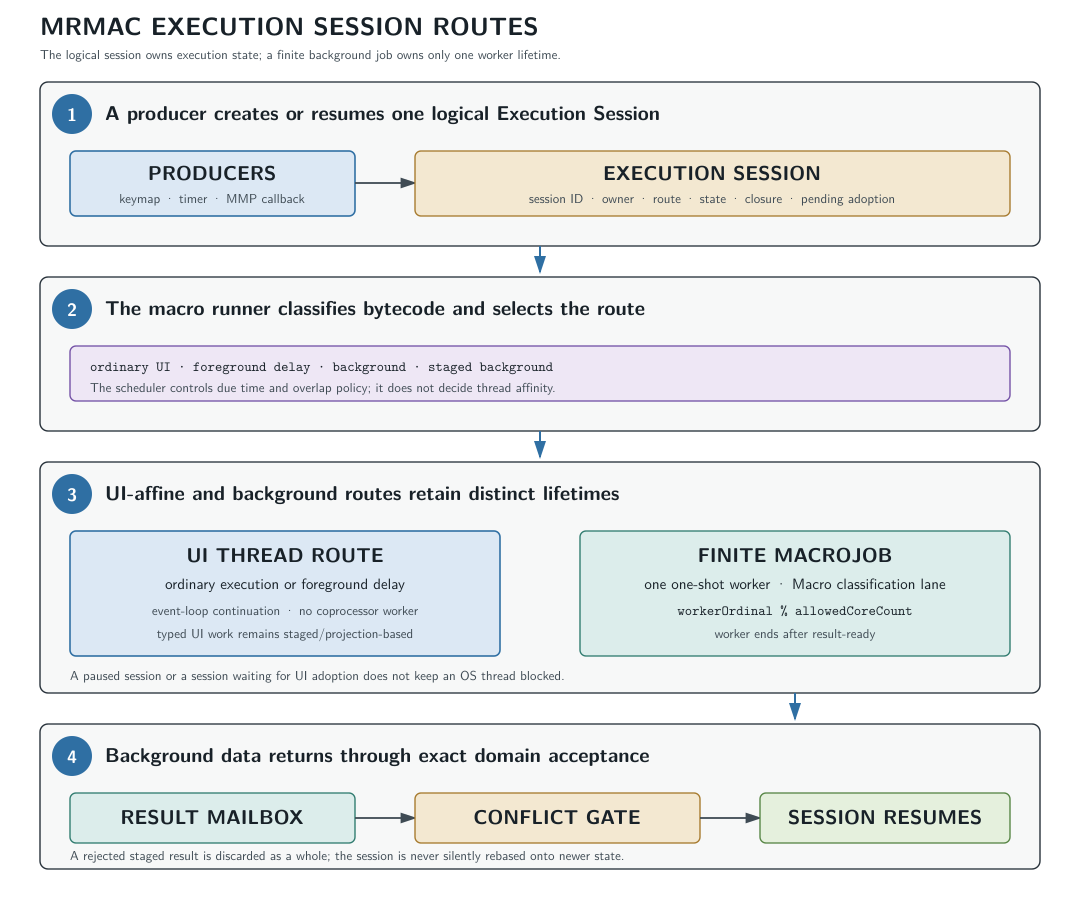
\includegraphics[width=\textwidth]{assets/mrmac-exec-session-scheduler-routes.pdf}
  \caption{Execution-session routing. UI-affine and foreground-delay work
  remain on the UI thread. Background and staged-background work enter the
  single-worker macro lane, whose worker is pinned round-robin to an available
  CPU core. A staged result returns through the mailbox for a domain-specific
  acceptance decision.}
  \label{fig:mrmac-session-routes}
\end{figure}

The clock thereby became a shared foundation for recurring closures, modeless
UI callbacks, execution status, and later the debugger. A scheduler that does
not blindly place a second due execution next to the first is not a
convenience-driven restriction. It protects retained UI state and external
work from overlaps that cannot be explained afterwards.

\chapter{Coprocessor, staging, and the UI thread}
\label{ch:macro-staging}

The VM must not alter a TVision view from a worker thread. For macro work that
is suitable for the background, it therefore produces a staging result: text
transactions, runtime state, and deferred UI commands are first collected as
data. Only the UI thread evaluates the commit conditions against the current
document and runtime state.

An accepted commit changes the model first and then provides the deferred UI
projection. A rejected commit is not partly repaired or rewritten for a newer
version. This boundary explains why the UI pump does not ``validate'' in a
general sense. It drains a bounded result mailbox; each result carries its own
domain-specific acceptance check.

This is what decoupling means technically in \mr{}: not arbitrary threads
being permitted to do things, but work whose result may become visible at an
explicit boundary with an accountable owner.

\chapter{MMP and a debugger for a real runtime}

MMP, the Modeless Macro Programs, were another point at which an apparently
quick shortcut was rejected. Macros were not given raw TVision pointers,
arbitrary paint callbacks, or a second event loop. Instead, they define
retained UI state in the VM K/V model; TVision projects that state as windows,
controls, and input. Timers use the session scheduler, and closing a window
removes its associated timers and callbacks with their owner.

The integrated \mrmac{} debugger is a consequence of that runtime
architecture. It offers breakpoints, pause, stepping, continue, cancellation,
variables, and watches not only for a synchronously started file. It works
with session identity and can therefore also account for Exec Sessions and
asynchronous closures. Source, debug state, watches, and output meet in a
Bento workspace without the debug view itself inventing execution truth.

A macro debugger that understood only the simple, straight-line path would be
cosmetic here. This debugger demonstrates that session, route, source map, and
runtime values are genuinely parts of one model.

\part{The editor as a personal environment}

\chapter{settings.mrmac: configuration as executable state}

\mr{} does not store its configuration as a JSON or YAML data heap.
\texttt{settings.mrmac} is controlled bootstrap source in the language that
belongs to the compiled application. The bootstrap reads the existing state,
checks and normalises it, drops unknown or obsolete ends, adds current defaults,
and writes canonical source with the current Build Epoch.

The file is not then the live runtime owner. The VM executes the startup
\texttt{MRSETUP} path; only the central in-memory settings state governs the
running application. This ``cutting off the old braid'' approach avoids an
ever-growing collection of compatibility lists. On loading, the past is
translated into a current, readable, executable form.

There are explicitly named transitional tensions, including keymap staging
while loading. It is not a hidden second authority, but a bounded exception
because serialisation accesses the canonical keymap model. \texttt{WORKSPACE},
too, is a protected extension of persistence, not an unnoticed part of the
canonical core settings contract.

\chapter{The settings bootstrap: canonical source and VM authority}

Figure~\ref{fig:settings-bootstrap-flow} is the technical spine of this
chapter. It begins with the actual entry condition, not with a save or backup:
the bootstrap ensures that a settings source exists. Each numbered phase names
the responsibility, data form, and authority boundary that the following
sections explain in detail.

\begin{figure}[htbp]
  \centering
  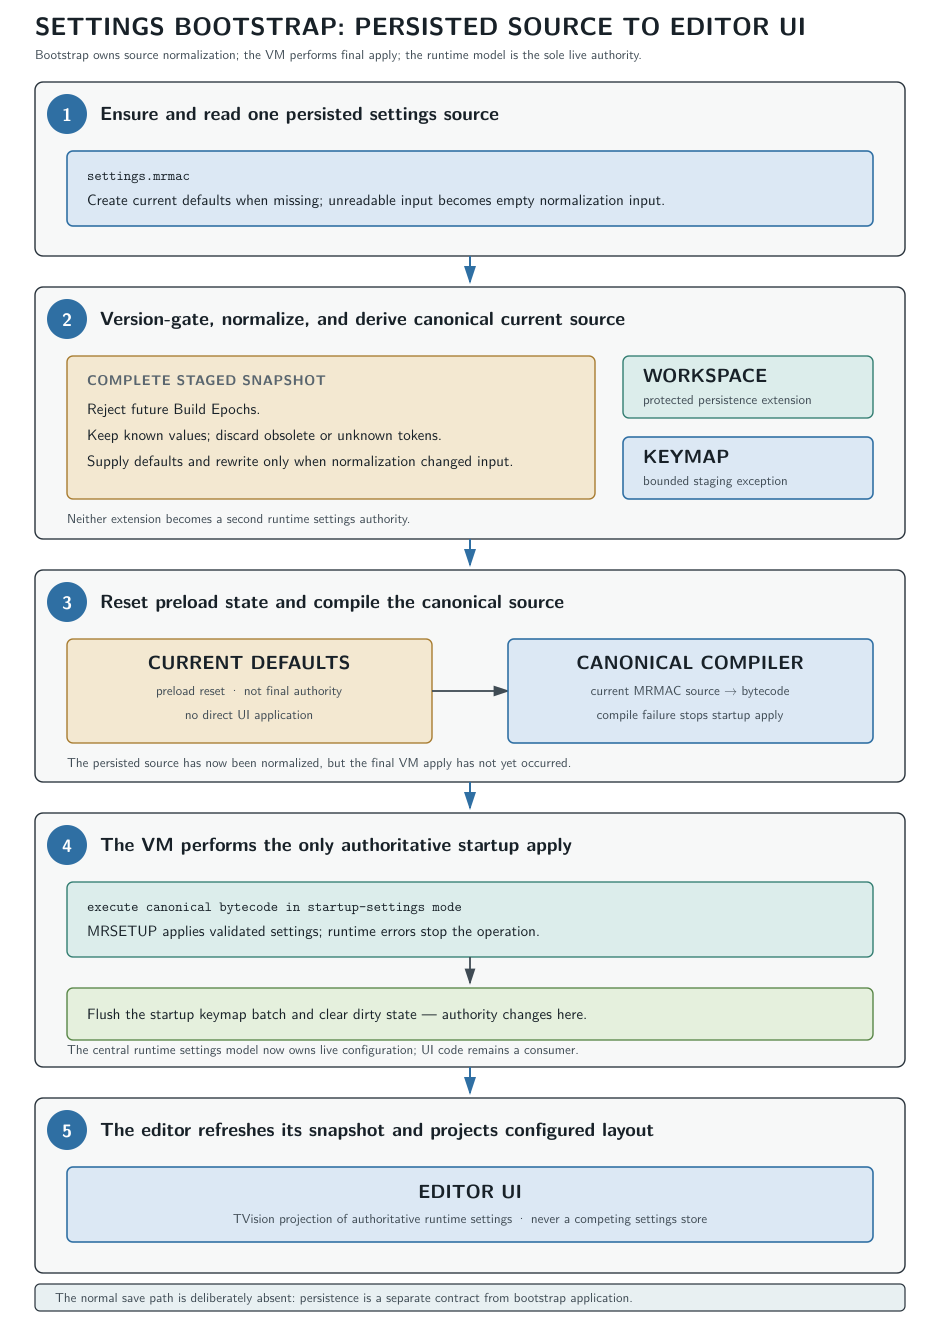
\includegraphics[width=0.82\textwidth]{assets/mr-settings-bootstrap-flow.pdf}
  \caption{VM-centred settings bootstrap. A persisted source is checked,
  normalised, and made canonical before the VM performs the final startup
  \texttt{MRSETUP} apply. Only the successful VM route makes the central
  runtime settings model authoritative; the editor UI consumes that model.}
  \label{fig:settings-bootstrap-flow}
\end{figure}

\chapter{Keymaps as a programmable input language}

The argument over efficient editor interaction does not end with a default.
WordStar, Emacs, and Nano are not folklore in \mr{}; they demonstrate that
interaction is part of a personal way of working. A profile contains
context-dependent canonical key tokens and bindings. The Key Manager makes
this a usable editor feature rather than a configuration-file trick: it lets a
user work with profiles and bindings, choose an action or macro target, and
record a sequence live in canonical keymap syntax. Invalid sequences,
collisions, and terminal/prefix conflicts are diagnosed before the profile
becomes live. The resolver then builds the Keymap Trie as the runtime
projection; the trie is not the feature's user interface, but the structure
that makes its input grammar decidable.

A sequence is not a hard-coded single keystroke. It is stored as a token
sequence and has no fixed length limit in the data model. The resolver may
hold a prefix open, but it forbids terminal/prefix collisions. Thus there is
no ambiguous waiting period in which a completed command might yet turn into a
longer one.

What matters most is the target of a binding. It may be a fast built-in action
or a file-qualified \mrmac{} macro. The user can therefore bind not just
\emph{Save} or \emph{Cursor Left}, but their own complex, reviewable automation
to their input language. This freedom is not unbounded: profile, context,
token parser, trie, and the distinction between action and macro give it a
form that can be understood.

\chapter{Profiles and automatic setup}

File-extension profiles associate one or more selectors with effective editing
settings, a window theme, and, where necessary, a compiler profile. A C++
project, a \LaTeX{} document, and a shell script thereby receive not only a
different colour, but an appropriate working environment. These profiles, too,
are described through \texttt{settings.mrmac}, not hidden in a second, loose
registry.

Compiler auto-setup extends the same idea. It finds known tools on
\texttt{PATH}, probes their version and characteristics, and creates or
completes profiles for toolchains that are actually present. That avoids empty
configuration forms without pretending to understand every possible build
system automatically. A profile remains visible and editable, and may include
build hooks and MRMAC actions.

\part{Syntax as a shared core}

\chapter{From an external generator to an integrated syntax model}

The first attempt to recognise \mrmac{} sources used Lex and Bison. That
approach proved outdated and did not provide a viable foundation for an editor
whose language knowledge must serve colouring, folding, and indentation at
the same time. The version history preserves at least the trace of removing
the Flex/Bison material; the engineering lesson matters more than the archive:
a parser generator does not itself solve the problem of an integrated,
incrementally usable editor model.

The present core combines classification by path, extension, and content probe
with shared line state and token runs, plus concrete rules for individual
languages. It deliberately does not claim to be a complete universal grammar.
Each language supplies its syntax state and token runs through the same
contract as the others; folding, outline, colouring, and indentation decisions
can reuse those results. \mrmac{} is consequently not a foreign C component
beside the editor, but a language in its own syntax model.

The current tree has 24 language modes, including Plain Text, not 384.
Automatic recognition combines file names, extensions, and a bounded content
probe. The number is smaller than the perceived breadth of the editor, but it
is the honest number. A later Tree-sitter trace was also removed from the
repository; the history proves the removal, but does not establish its exact
reason without further sources. This manual does not invent one afterwards.

\chapter{Trainers: the workbench for language features}

The trainers are not machine learning. They are a workbench on which language
rules become visible, repeatable, and discussable against real examples. The
fold trainer automatically classifies an input when needed and emits its fold
structure as numbered ASCII. The outline trainer uses the same fold scan to
produce the outline.

The indent trainer goes further. It creates a real \texttt{MRFileEditor},
varies language, indentation style, UI style, and tab treatment, and simulates
Enter and Smart Undent. Its strict pass/fail expectations therefore exercise
production paths rather than an independently invented test semantics.

The trainers do not prove the entire visible behaviour under load; they are no
replacement for UI or coprocessor checks. They do secure the exact semantic
question that they show: which structure, outline element, and indentation
decision follows from this text? That is valuable testability because it is
made of the same language as the editor feature.

\part{Spaces and the Unix world}

\chapter{Virtual desktops and resumable workspaces}

A terminal editor need not be reduced to a single document window. \mr{}
assigns every desktop-capable window to a virtual desktop. When changing
desktops, windows on the other desktop are hidden, not destroyed; focus,
geometry, and state remain intact. Windows can be moved, minimised, tiled, and
cascaded without those desktop operations needing to know the domain nature of
an editor, a Bento view, or a modeless macro window.

A workspace makes this spatial working state recoverable. It stores, among
other things, URLs, window geometry, cursor positions, virtual desktop,
minimised and restore state, and Bento snapshots for suitable windows. Autoload
and autosave do not turn it into an all-powerful persistence layer; they make
it a deliberately bounded continuation of personal work.

The result is a TUI workspace in which many windows need not form an
unmanageable parade. They can live on virtual desktops and reappear in a
workspace exactly where work was interrupted.

\chapter{MFS and Acquire: Unix output as working material}

Multi-file search and multi-file replace combine recursive file work with
PCRE2 and can be restricted to the workspace. This is not merely a search box
with a different file dialog. It is a bridge between the open workspace and
the file tree.

Acquire follows another, particularly terminal-native idea. \mr{} runs a
shell command out of sight, reads its standard output, and interprets each line
as a candidate readable path. Candidates are resolved and deduplicated; the
user may open or load selected files or every discovered file. Acquire is
therefore not the uncritical insertion of arbitrary pipe bytes into a buffer.
It turns Unix tools into an understandable file selection.

\part{Decisions that left traces}

\chapter{The Hex restart and the LSP train}

The first Hex integration was discarded. Its lesson was specific: a Hex view
does not belong as a special branch in a generic BentoBox; it needs neither an
exception to the normal pane lifetime nor a self-drawn frame. Restarting it as
\texttt{MRBentoHexEditor}, with six ordinary pane windows, shared byte-cursor
logic, and the same document basis, was not cosmetic refactoring. It restored
clear responsibility.

The LSP train was more painful. Two attempts consumed weeks; the architecture
could not be shaped into a viable editor feature. The history ultimately
records the removal of the LSP material in a large rollback. This is not a
claim that LSP is inherently bad. It is the specific conclusion that an
external IDE model could not be integrated with adequate clarity and benefit
into this project's existing runtime, UI, and working model.

Both stories belong in the manual because discarding work can be a technical
ability. A system remains coherent not by saving every line once written, but
by being able to remove the wrong boundaries again.

\chapter{Observability, not wishful thinking}

The enwik9 measurement, K/V instrumentation, performance panels, execution
status, live log, and trainers have one purpose in common: they make technical
claims open to challenge. A slow operation should not end as a vague user
report, but become visible as a measurable duration, request, result, or
discarded version.

The build belongs to this story as well. It orchestrates the TVision upstream,
the MRMAC compiler, training programs, regression checks, and manuals. A clean
rebuild is not a ritual; it tests whether the delivery form claimed by the
repository can actually be produced from its source.

\backmatter
\chapter*{Outlook}
\addcontentsline{toc}{chapter}{Outlook}

The technical centre of \mr{} is not one individual trick. It is the repeated
application of the same attitude: do not copy original data unnecessarily,
decouple derived work from interaction, give truth one unambiguous owner, and
place extensibility under the same boundaries as built-in code. This is why a
gigabyte document can become useful immediately, a Braille minimap can exist
in a console, a user can program an input language, and a deferred macro can
remain debuggable.

\end{document}
